
Two concepts were initially explored, but rejected for various reasons. The first concept was a shape-memory-alloy (SMA) actuator
that could be moved over a perch and into a lock that would hold it in place. The actuator would consist of 3 individual SMA wires
that could each move the device into a home, reaching, or latched position. The concept is illustrated in Fig. \ref{fig:latch-sma}.
This concept was rejected due to concerns over available time and the author's lack of familiarity with SMA materials.

\begin{figure}[H]
    \centering
    \begin{subfigure}[b]{\textwidth}
        \begin{subfigure}[b]{0.32\textwidth}
            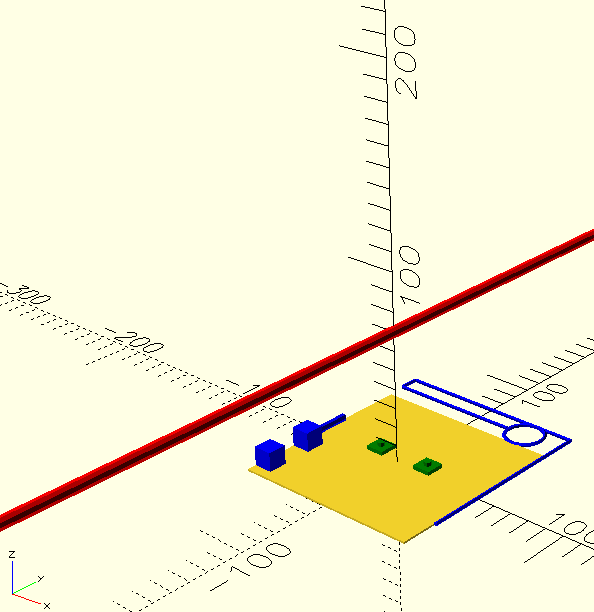
\includegraphics[width=\textwidth]{sections/methods/sma-concept-home.png}
            \caption{The device in its home position, with the SMA bundle coiled out of the camera's view.}
            \label{fig:latch-sma:home}
        \end{subfigure}
        \hfill
        \begin{subfigure}[b]{0.32\textwidth}
            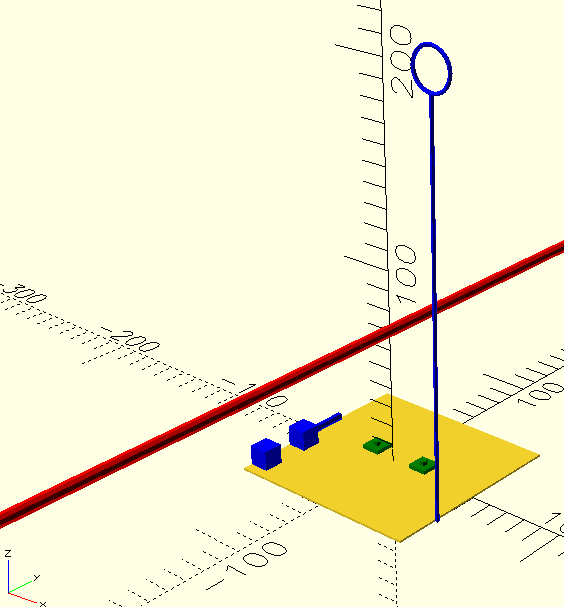
\includegraphics[width=\textwidth]{sections/methods/sma-concept-raised.png}
            \caption{The device with the SMA bundle extended, ready to grasp a perch.}
            \label{fig:latch-sma:raised}
        \end{subfigure}
        \hfill
        \begin{subfigure}[b]{0.32\textwidth}
            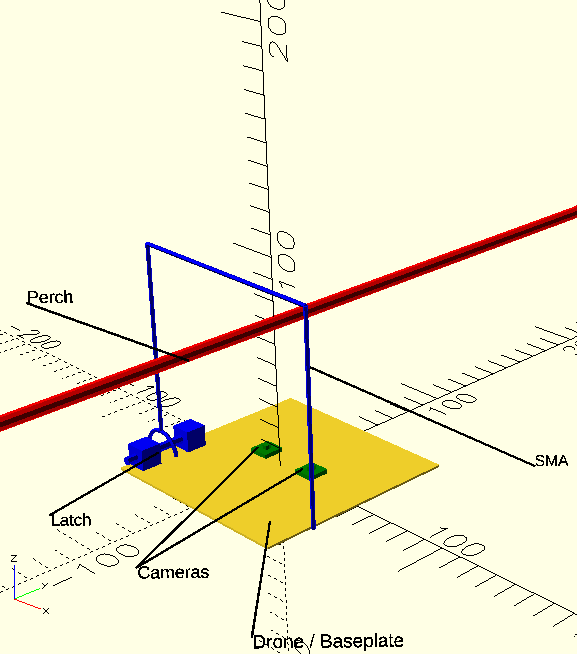
\includegraphics[width=\textwidth]{sections/methods/sma-concept-latched.png}
            \caption{The device with the SMA bundle wrapped over a perch, and the latch engaged.}
            \label{fig:latch-sma:latched}
        \end{subfigure}
    \end{subfigure}
    \caption{Rendered sketch of the shape-memory-alloy based grasper concept in 3 stages of grasping. The base or drone airframe is shown 
    in yellow, camera locations in green, and the target perch is shown in red. In blue is the grasping mechanism, consisting of a bundle of 
    SMA wire actuators and a loop on the right, and on the left a latch mechanism that holds the SMA in place once it is grasped.}
    \label{fig:latch-sma}
\end{figure}

A similar concept that replaced the SMA mechanism with a cable-actuated flexible grasper was prototyped. The intent was that
the grasper would wrap over a perch and into a latch similarly to the SMA device, but with a grasper 3D printed from thermoplastic
polyurethane (TPU) filament and driven by servo motors via cables.
This design was rejected because the hobby servos used could not provide enough torque to bend the grasper as needed, 
and the flexibility combined with the elasticity of the cable drive prevented the device
from achieving sufficient repeatability in position control. Fig. \ref{fig:latch-cable} shows this prototype device.

\begin{figure}[H]
    \centering
    \begin{subfigure}[b]{\textwidth}
        \begin{subfigure}[b]{0.45\textwidth}
            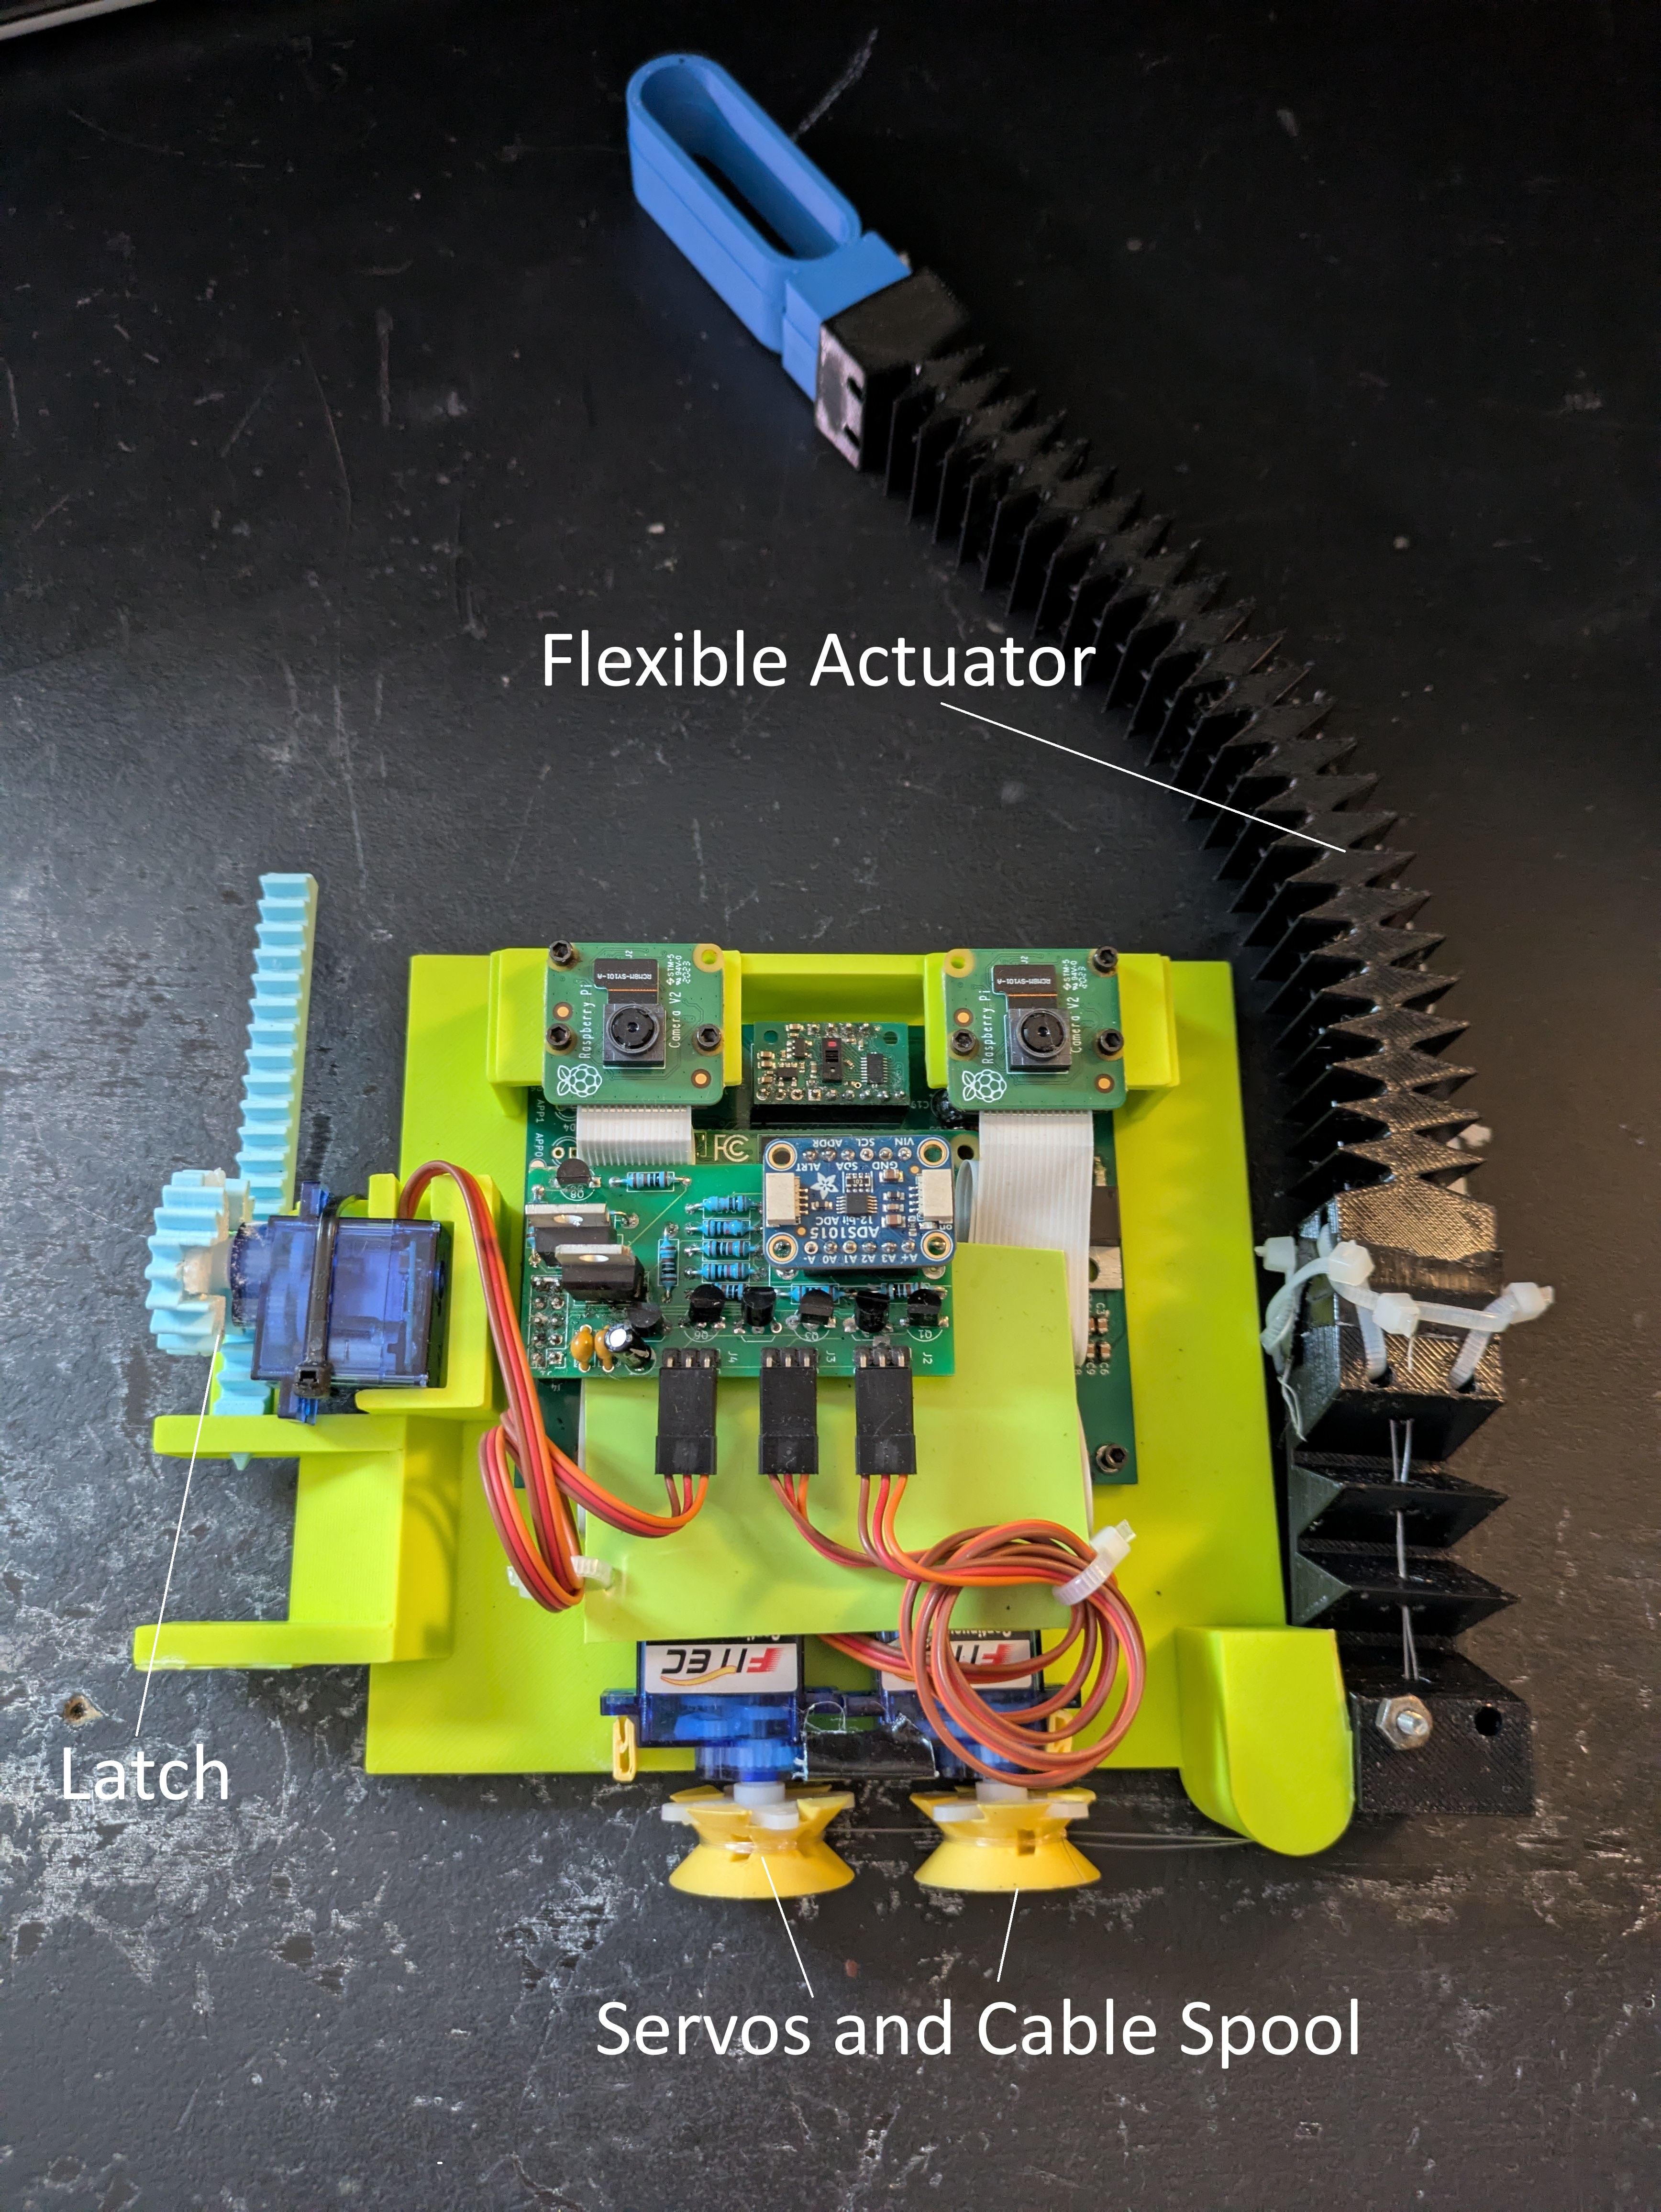
\includegraphics[width=\textwidth]{sections/methods/flex-open.jpg}
            \caption{The grasper in its open, resting state.}
            \label{fig:latch-cable:open}
        \end{subfigure}
        \hfill
        \begin{subfigure}[b]{0.45\textwidth}
            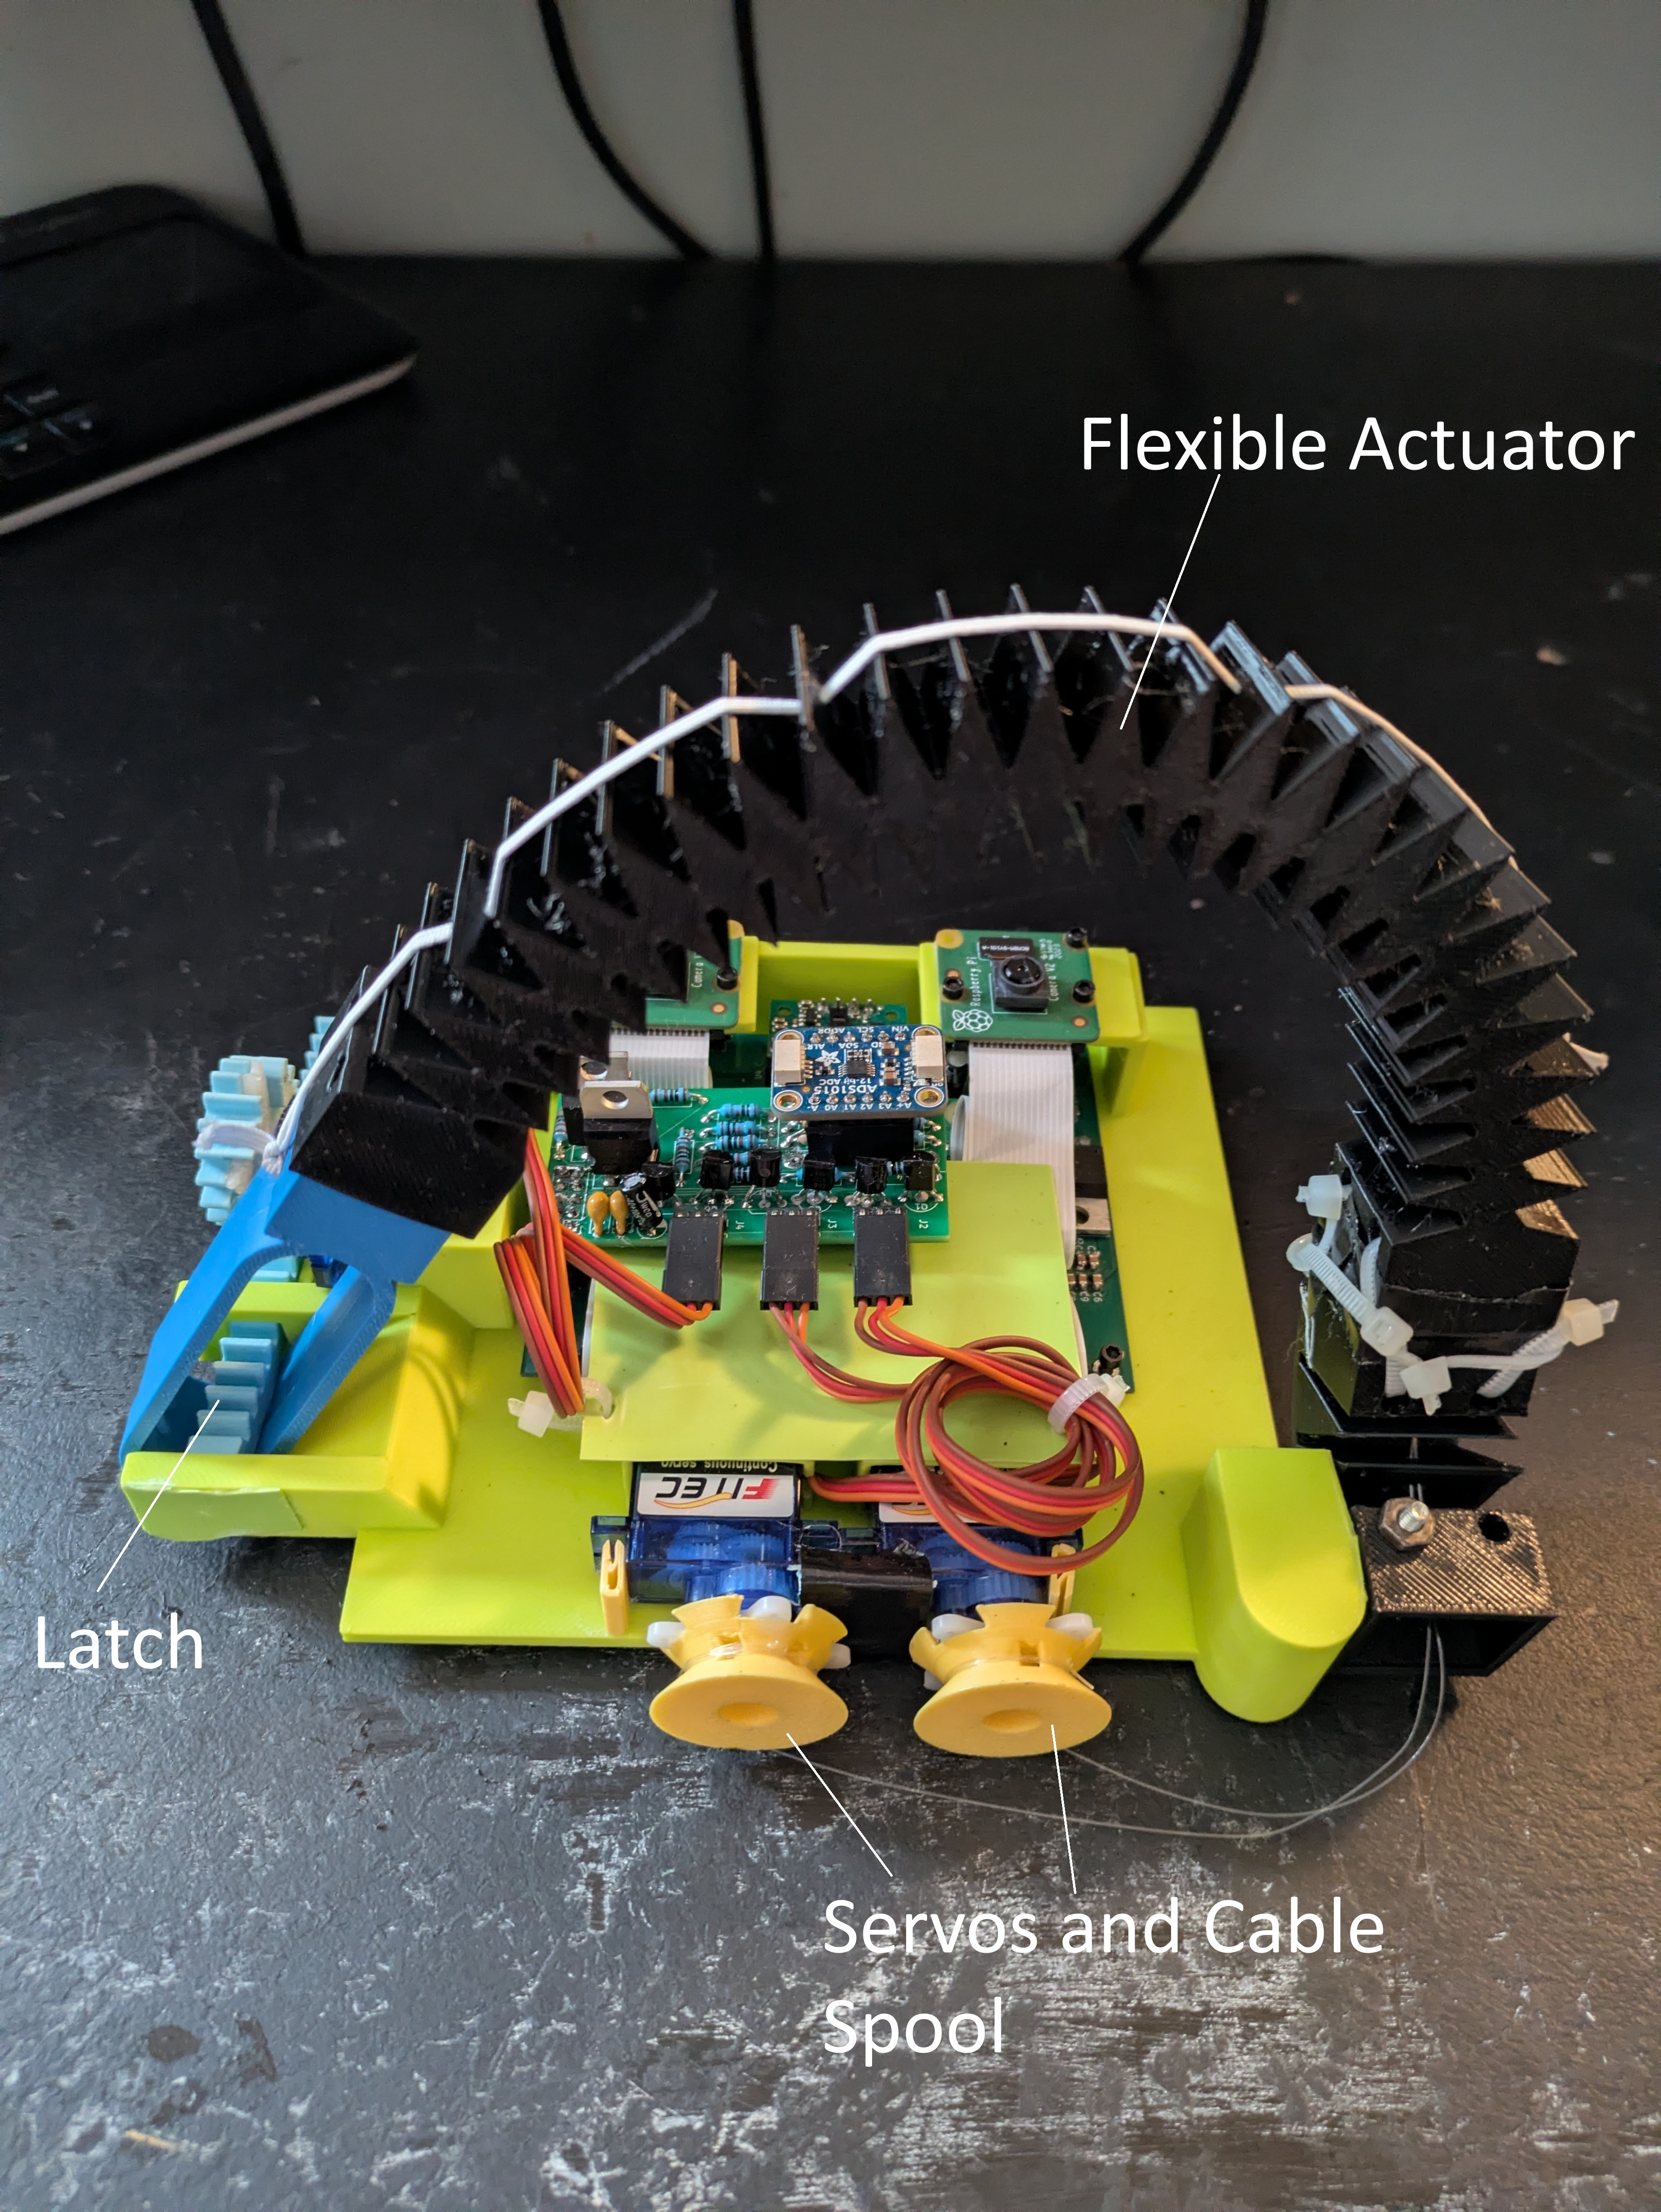
\includegraphics[width=\textwidth]{sections/methods/flex-closed.jpg}
            \caption{The grasper in its closed state.}
            \label{fig:latch-cable:closed}
        \end{subfigure}
    \end{subfigure}
    \caption{The cable-actuated flexible grasper concept, which was prototyped but rejected 
    due to the hobby servo's inability to produce sufficient tension, and the low precision of 
    the positioning of the actuator.}
    \label{fig:latch-cable}
\end{figure}